\chapter{IMPLEMENTATION}

This chapter details the concrete programmatic implementation of the end-to-end churn prediction and segmentation framework, describing file organization, code execution workflows, preprocessing mechanisms, and representative algorithm listings.

\section{DATASET ACQUISITION}
The dataset was obtained from the IBM Cognos Analytics accelerator repository as a structured CSV archive titled \texttt{WA\_Fn-UseC\_-Telco-Customer-Churn.csv}. The project repository manages raw data ingestion through \texttt{src/data\_loader.py}. Upon ingestion, an automated audit script validates that exactly \datasetTotalRows{} rows and \datasetTotalCols{} columns exist, verifies zero duplicate customer records, and flags the 11 instances of whitespace in \texttt{TotalCharges}. An automated data dictionary and audit summary are generated in \texttt{results/dataset\_audit.json} and \texttt{results/data\_dictionary.csv}.

\section{DATA PRE-PROCESSING}
Data cleaning and transformation are implemented within \texttt{src/preprocessing.py}. The pipeline isolates the target vector $y = \texttt{Churn}$ and ID vector $\texttt{customerID}$, leaving 19 feature columns. Preprocessing is implemented via an integrated scikit-learn \texttt{ColumnTransformer}:
\begin{itemize}
    \item \textbf{Numerical Transformers:} \texttt{tenure}, \texttt{MonthlyCharges}, and \texttt{TotalCharges} pass through \texttt{SimpleImputer(strategy='median')} followed by \texttt{StandardScaler()}.
    \item \textbf{Categorical Transformers:} The 16 categorical features pass through \texttt{SimpleImputer(strategy='most\_frequent')} followed by \texttt{OneHotEncoder(handle\_unknown='ignore', sparse\_output=False)}.
\end{itemize}
To guarantee that no test-set information bleeds into training statistics, the transformer is fitted strictly using \texttt{preprocessor.fit(X\_train)}, and the fitted object is serialized to \texttt{models/preprocessor.joblib}.

\section{FEATURE ANALYSIS AND EXPLORATORY VISUALIZATIONS}
Exploratory data analysis is implemented in \texttt{src/eda.py}. All visualizations are saved at 300 DPI directly to \texttt{reports/figures/} and \texttt{results/figures/}. Key exploratory distributions are depicted in Figure~\ref{fig:eda_contract_tenure}.

\begin{figure}[H]
    \centering
    \begin{subfigure}[b]{0.48\textwidth}
        \centering
        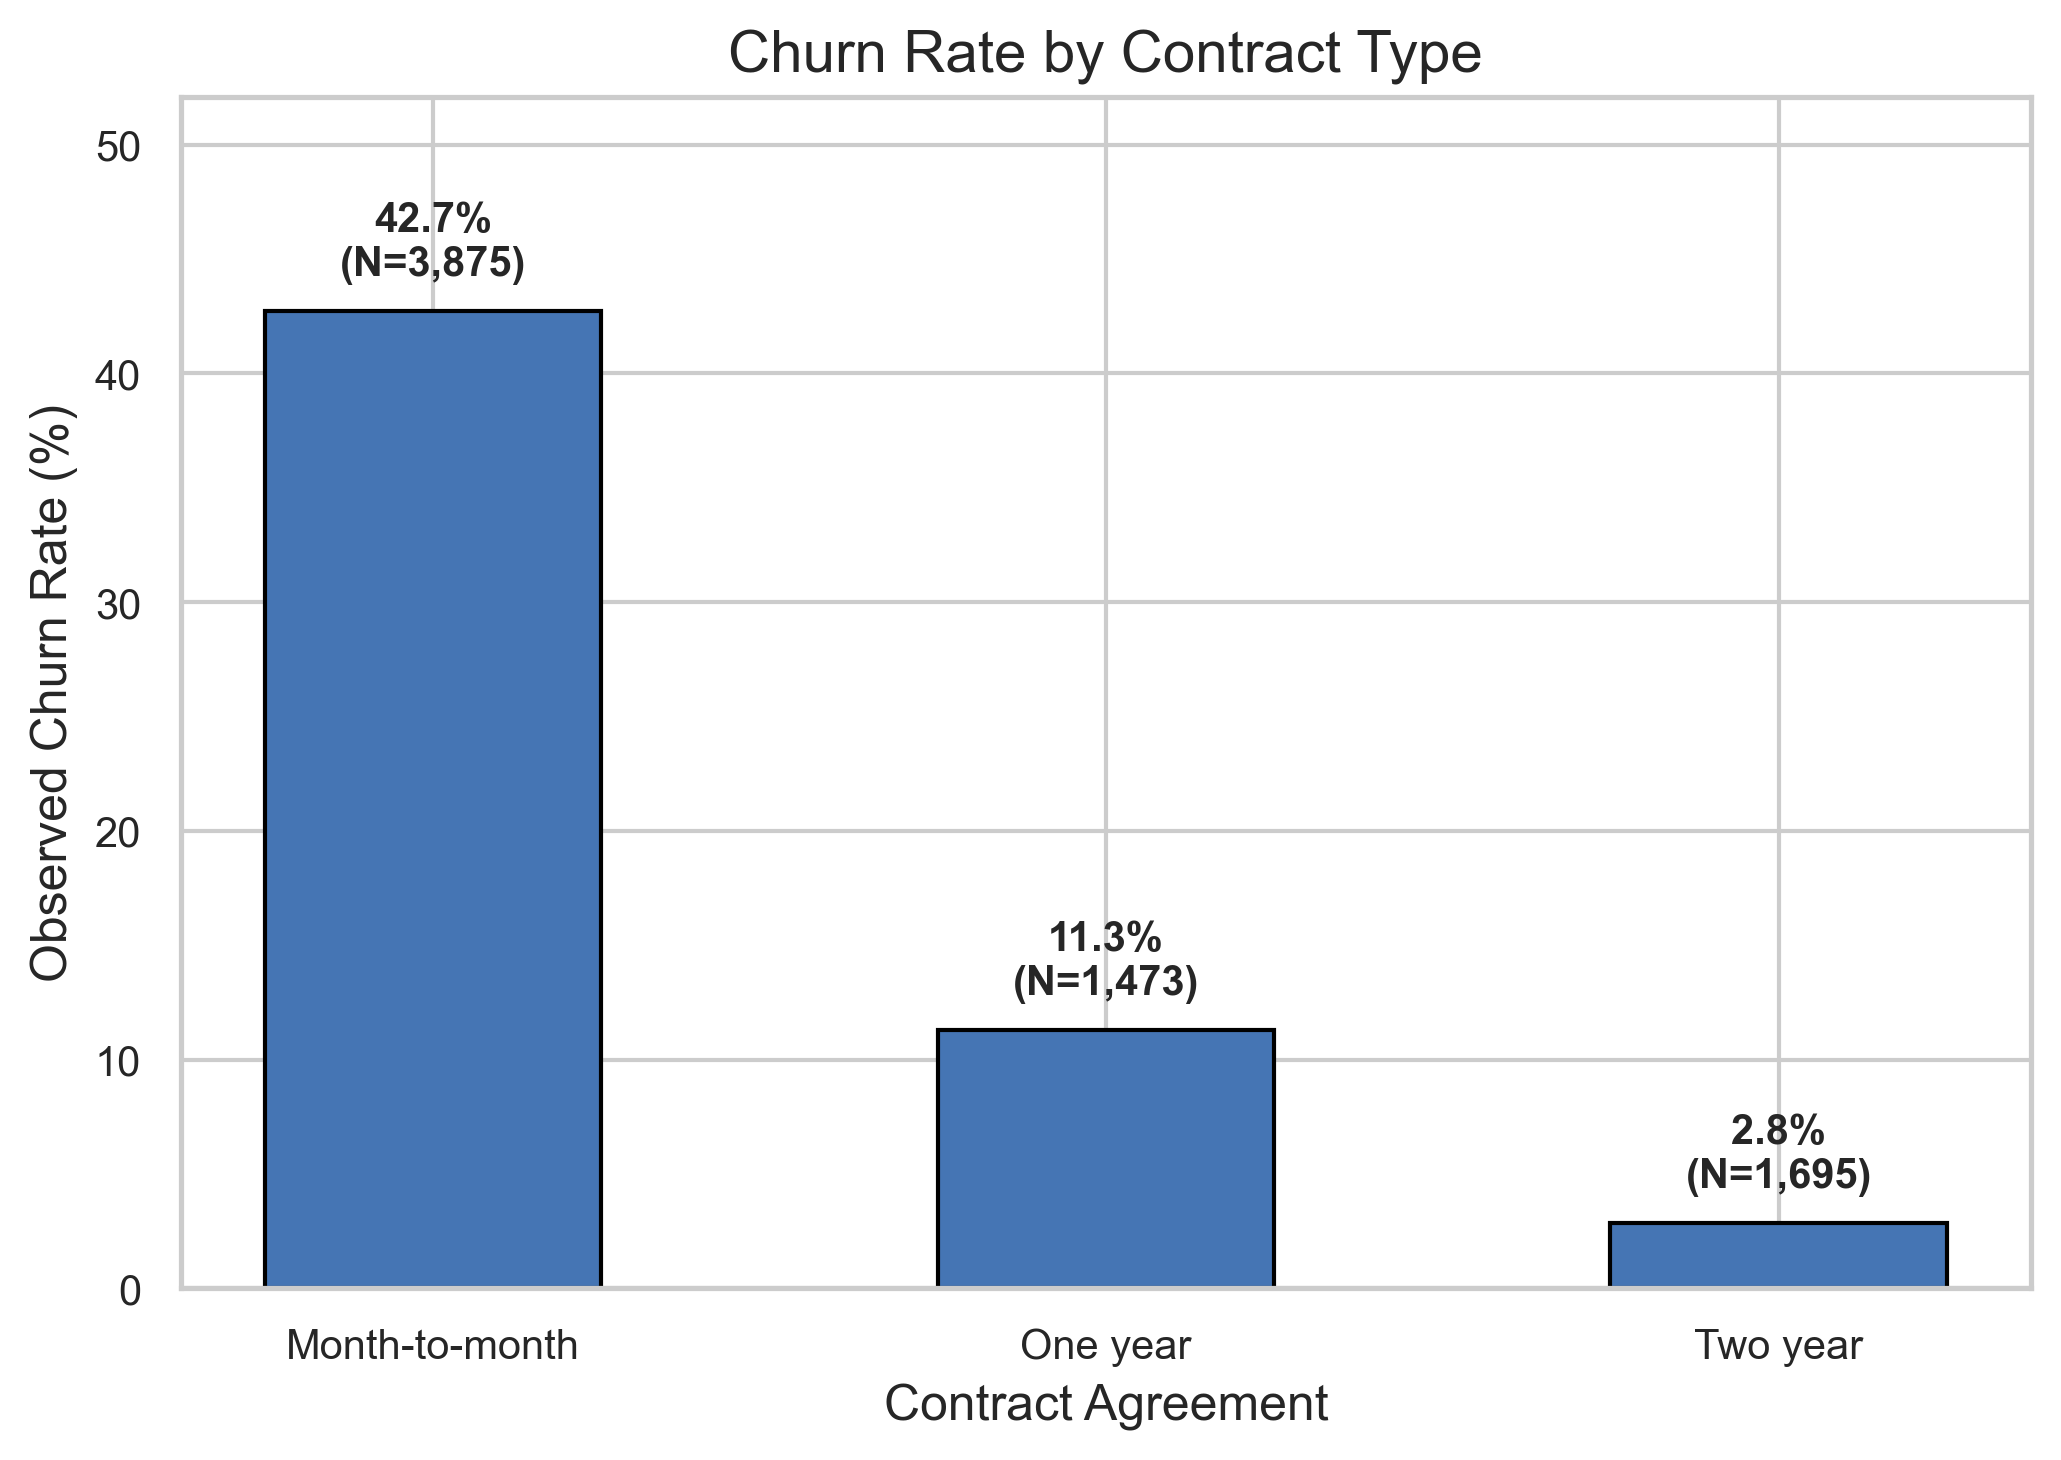
\includegraphics[width=\textwidth]{figures/eda_02_churn_by_contract.png}
        \caption{Churn Rate by Contract Commitment}
        \label{fig:eda_contract}
    \end{subfigure}
    \hfill
    \begin{subfigure}[b]{0.48\textwidth}
        \centering
        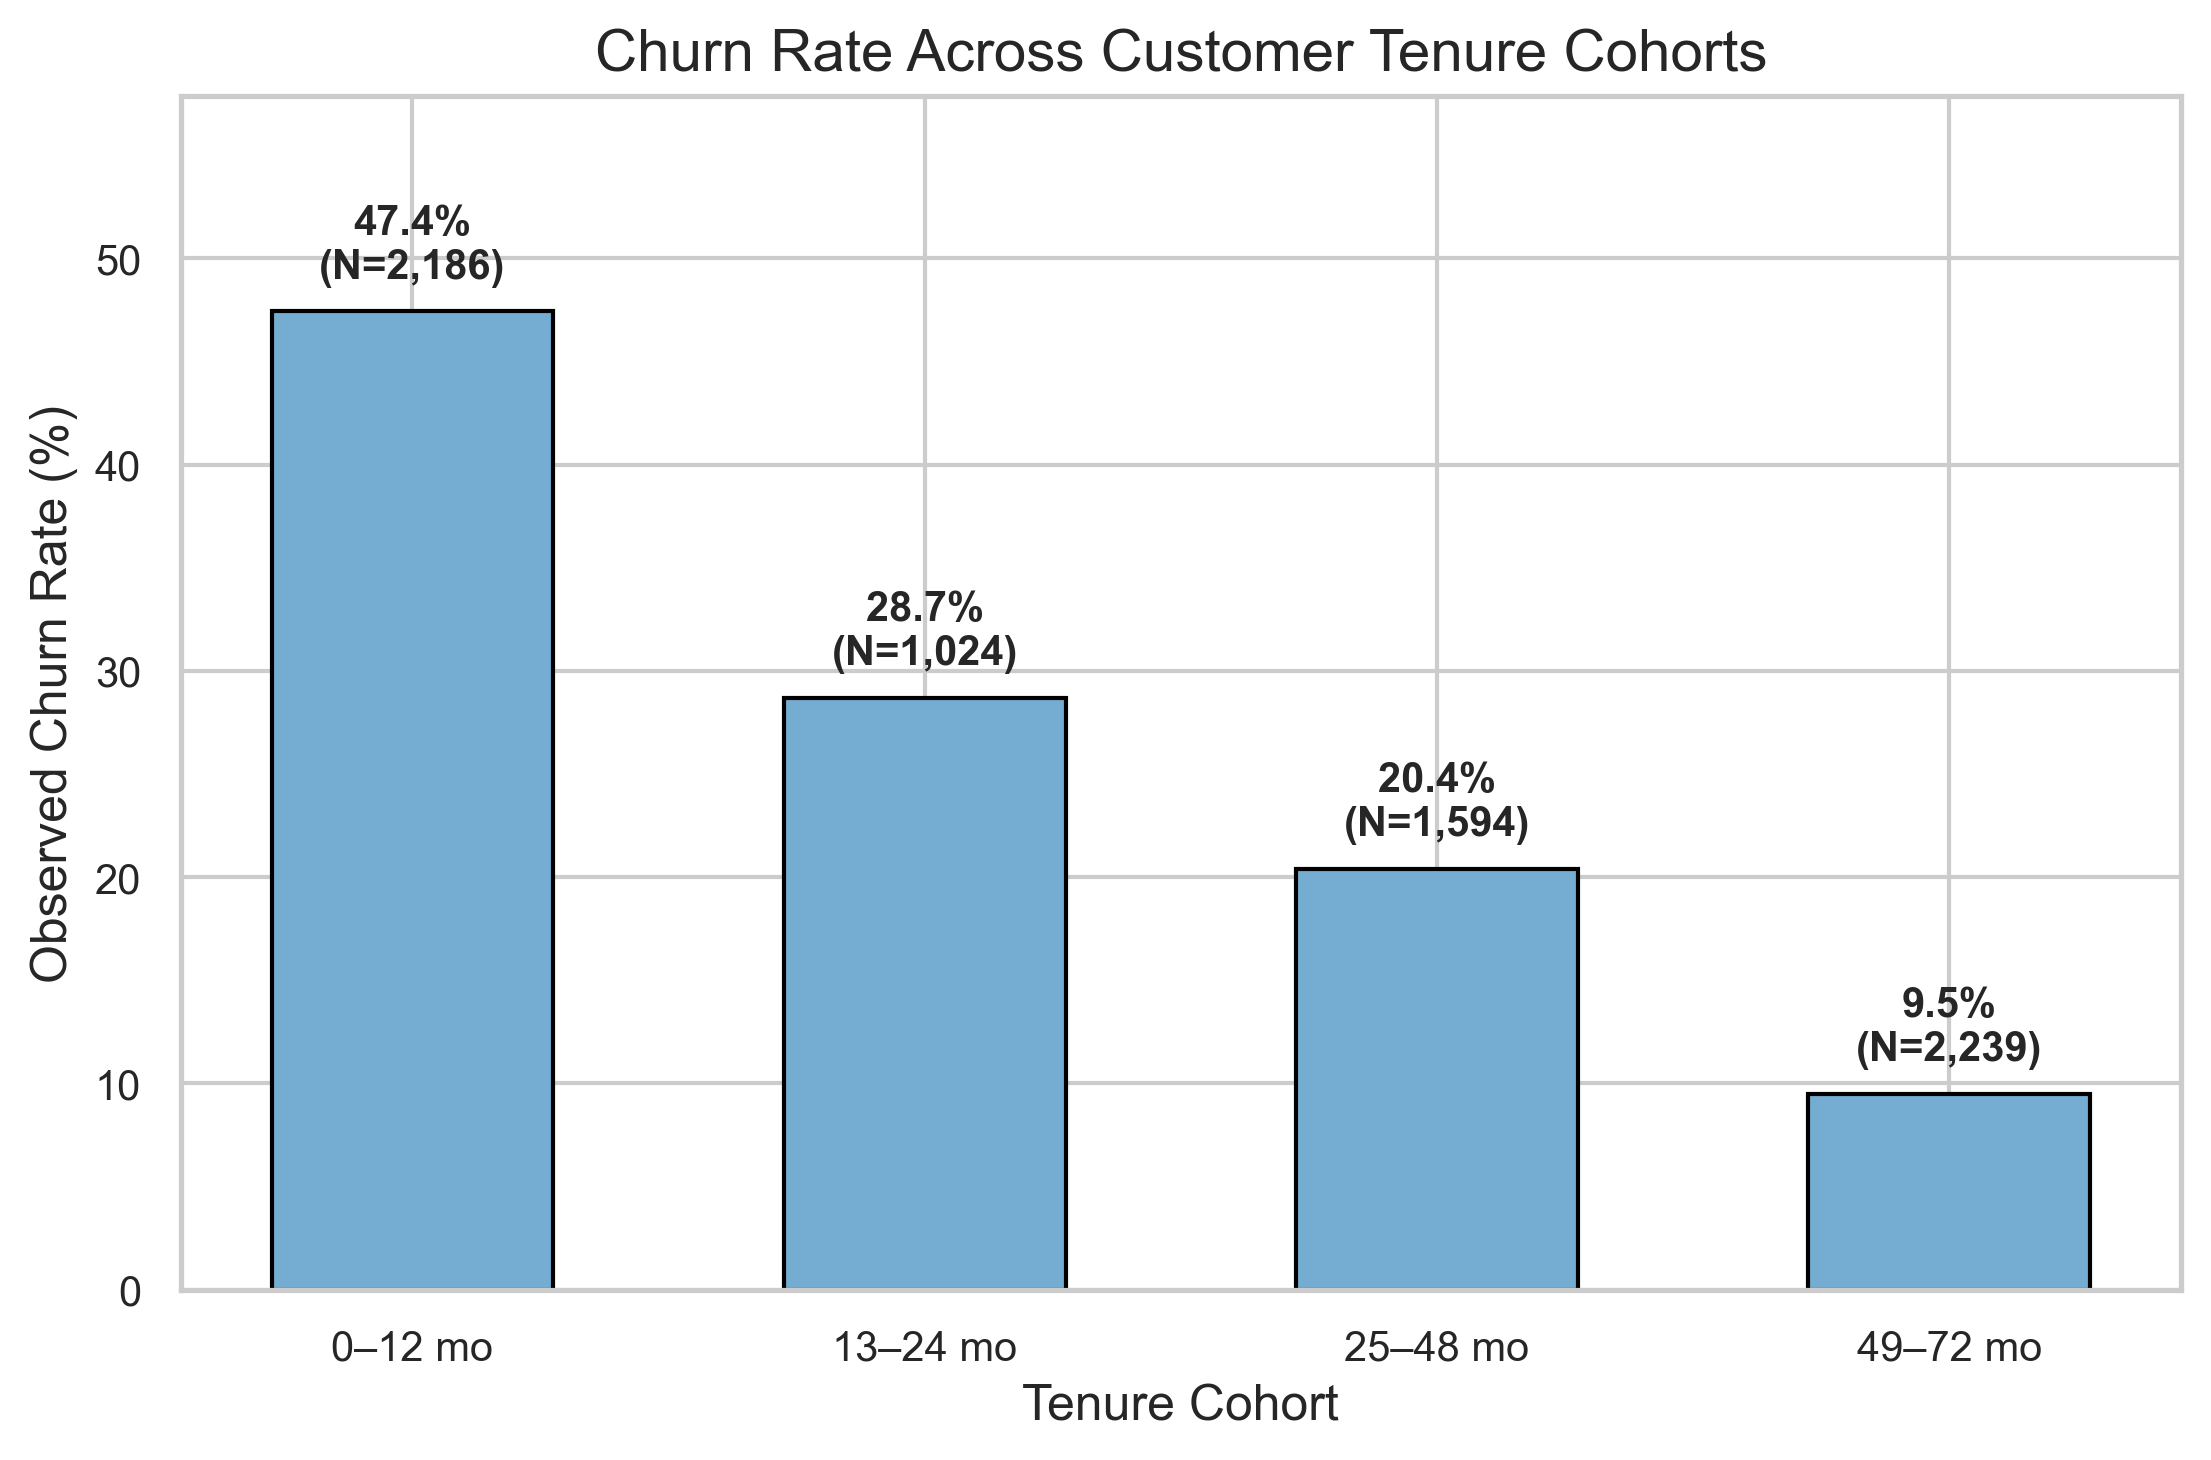
\includegraphics[width=\textwidth]{figures/eda_03_churn_by_tenure_group.png}
        \caption{Churn Rate across Tenure Cohorts}
        \label{fig:eda_tenure}
    \end{subfigure}
    \caption{Exploratory Analysis Demonstrating Structural Contract and Tenure Churn Disparities}
    \label{fig:eda_contract_tenure}
\end{figure}

The exploratory figures reveal that subscribers enrolled in month-to-month contracts experience a churn rate of 42.7\%, whereas subscribers committing to two-year contracts experience a churn rate of merely 2.8\%. Similarly, customers within their first 12 months of service exhibit a 47.7\% churn rate, which progressively diminishes to 6.6\% for subscribers retained beyond 48 months.

Figure~\ref{fig:eda_charges_payment} examines the density distribution of monthly billing charges and payment settlement methods.

\begin{figure}[H]
    \centering
    \begin{subfigure}[b]{0.48\textwidth}
        \centering
        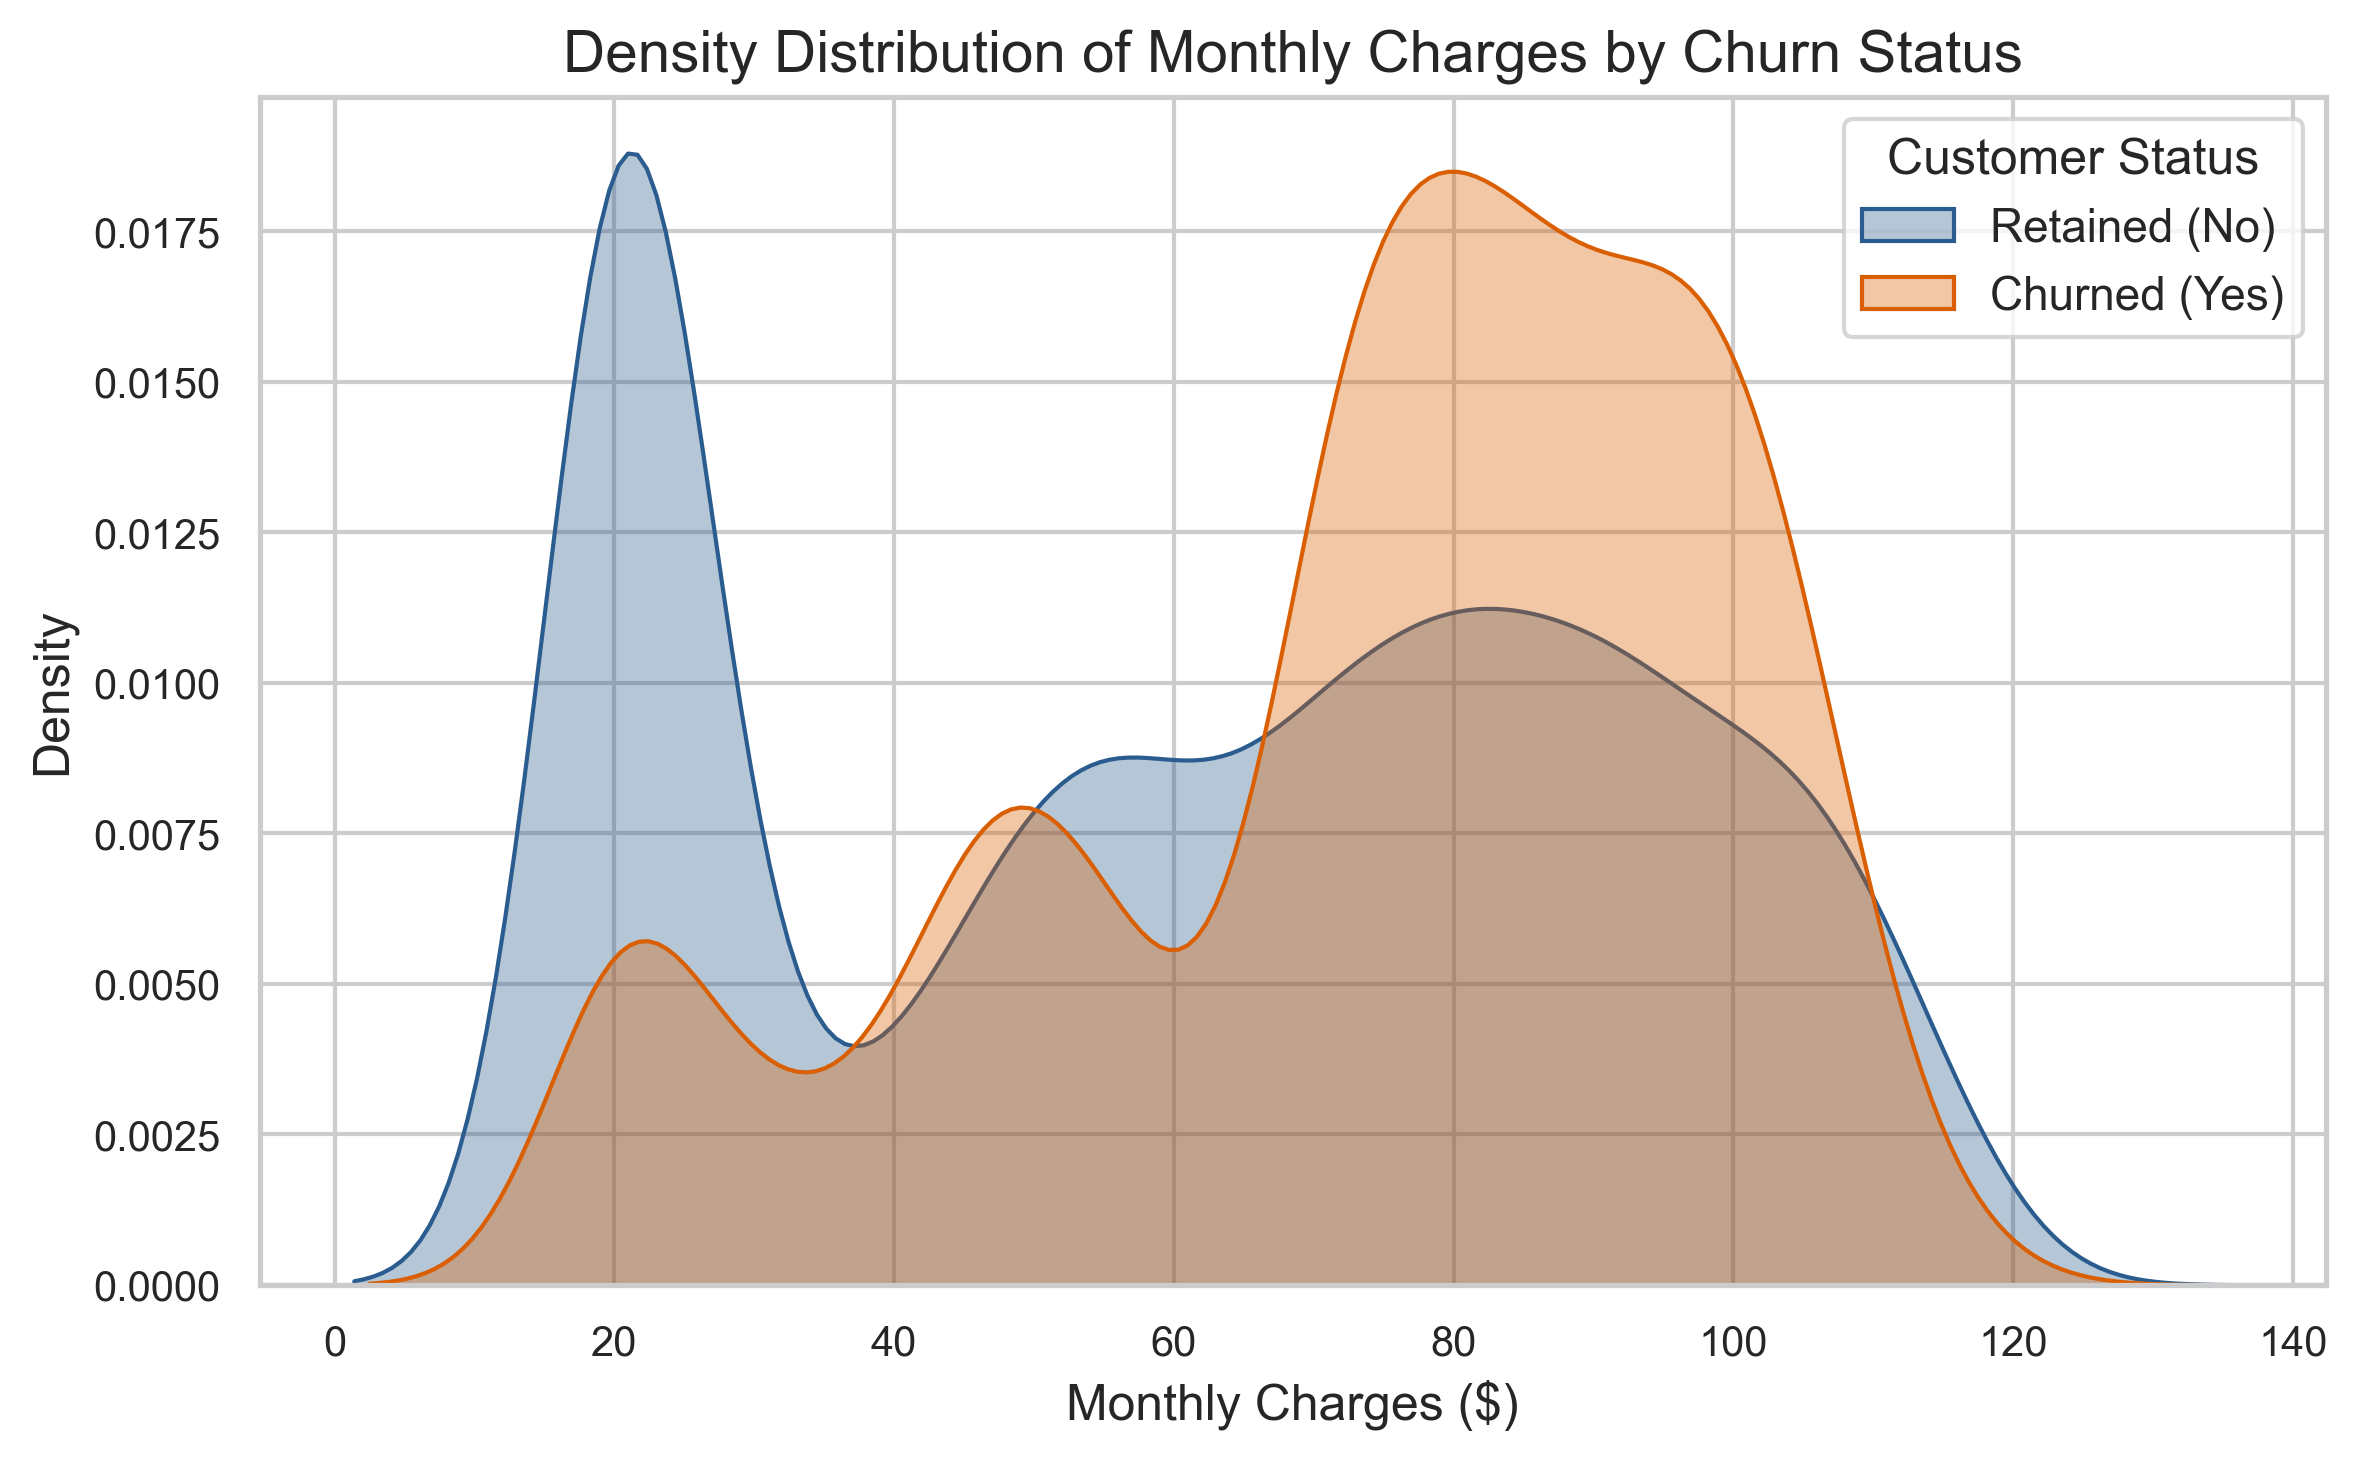
\includegraphics[width=\textwidth]{figures/eda_04_monthly_charges_distribution.png}
        \caption{Density of Monthly Charges by Churn Status}
        \label{fig:eda_monthly}
    \end{subfigure}
    \hfill
    \begin{subfigure}[b]{0.48\textwidth}
        \centering
        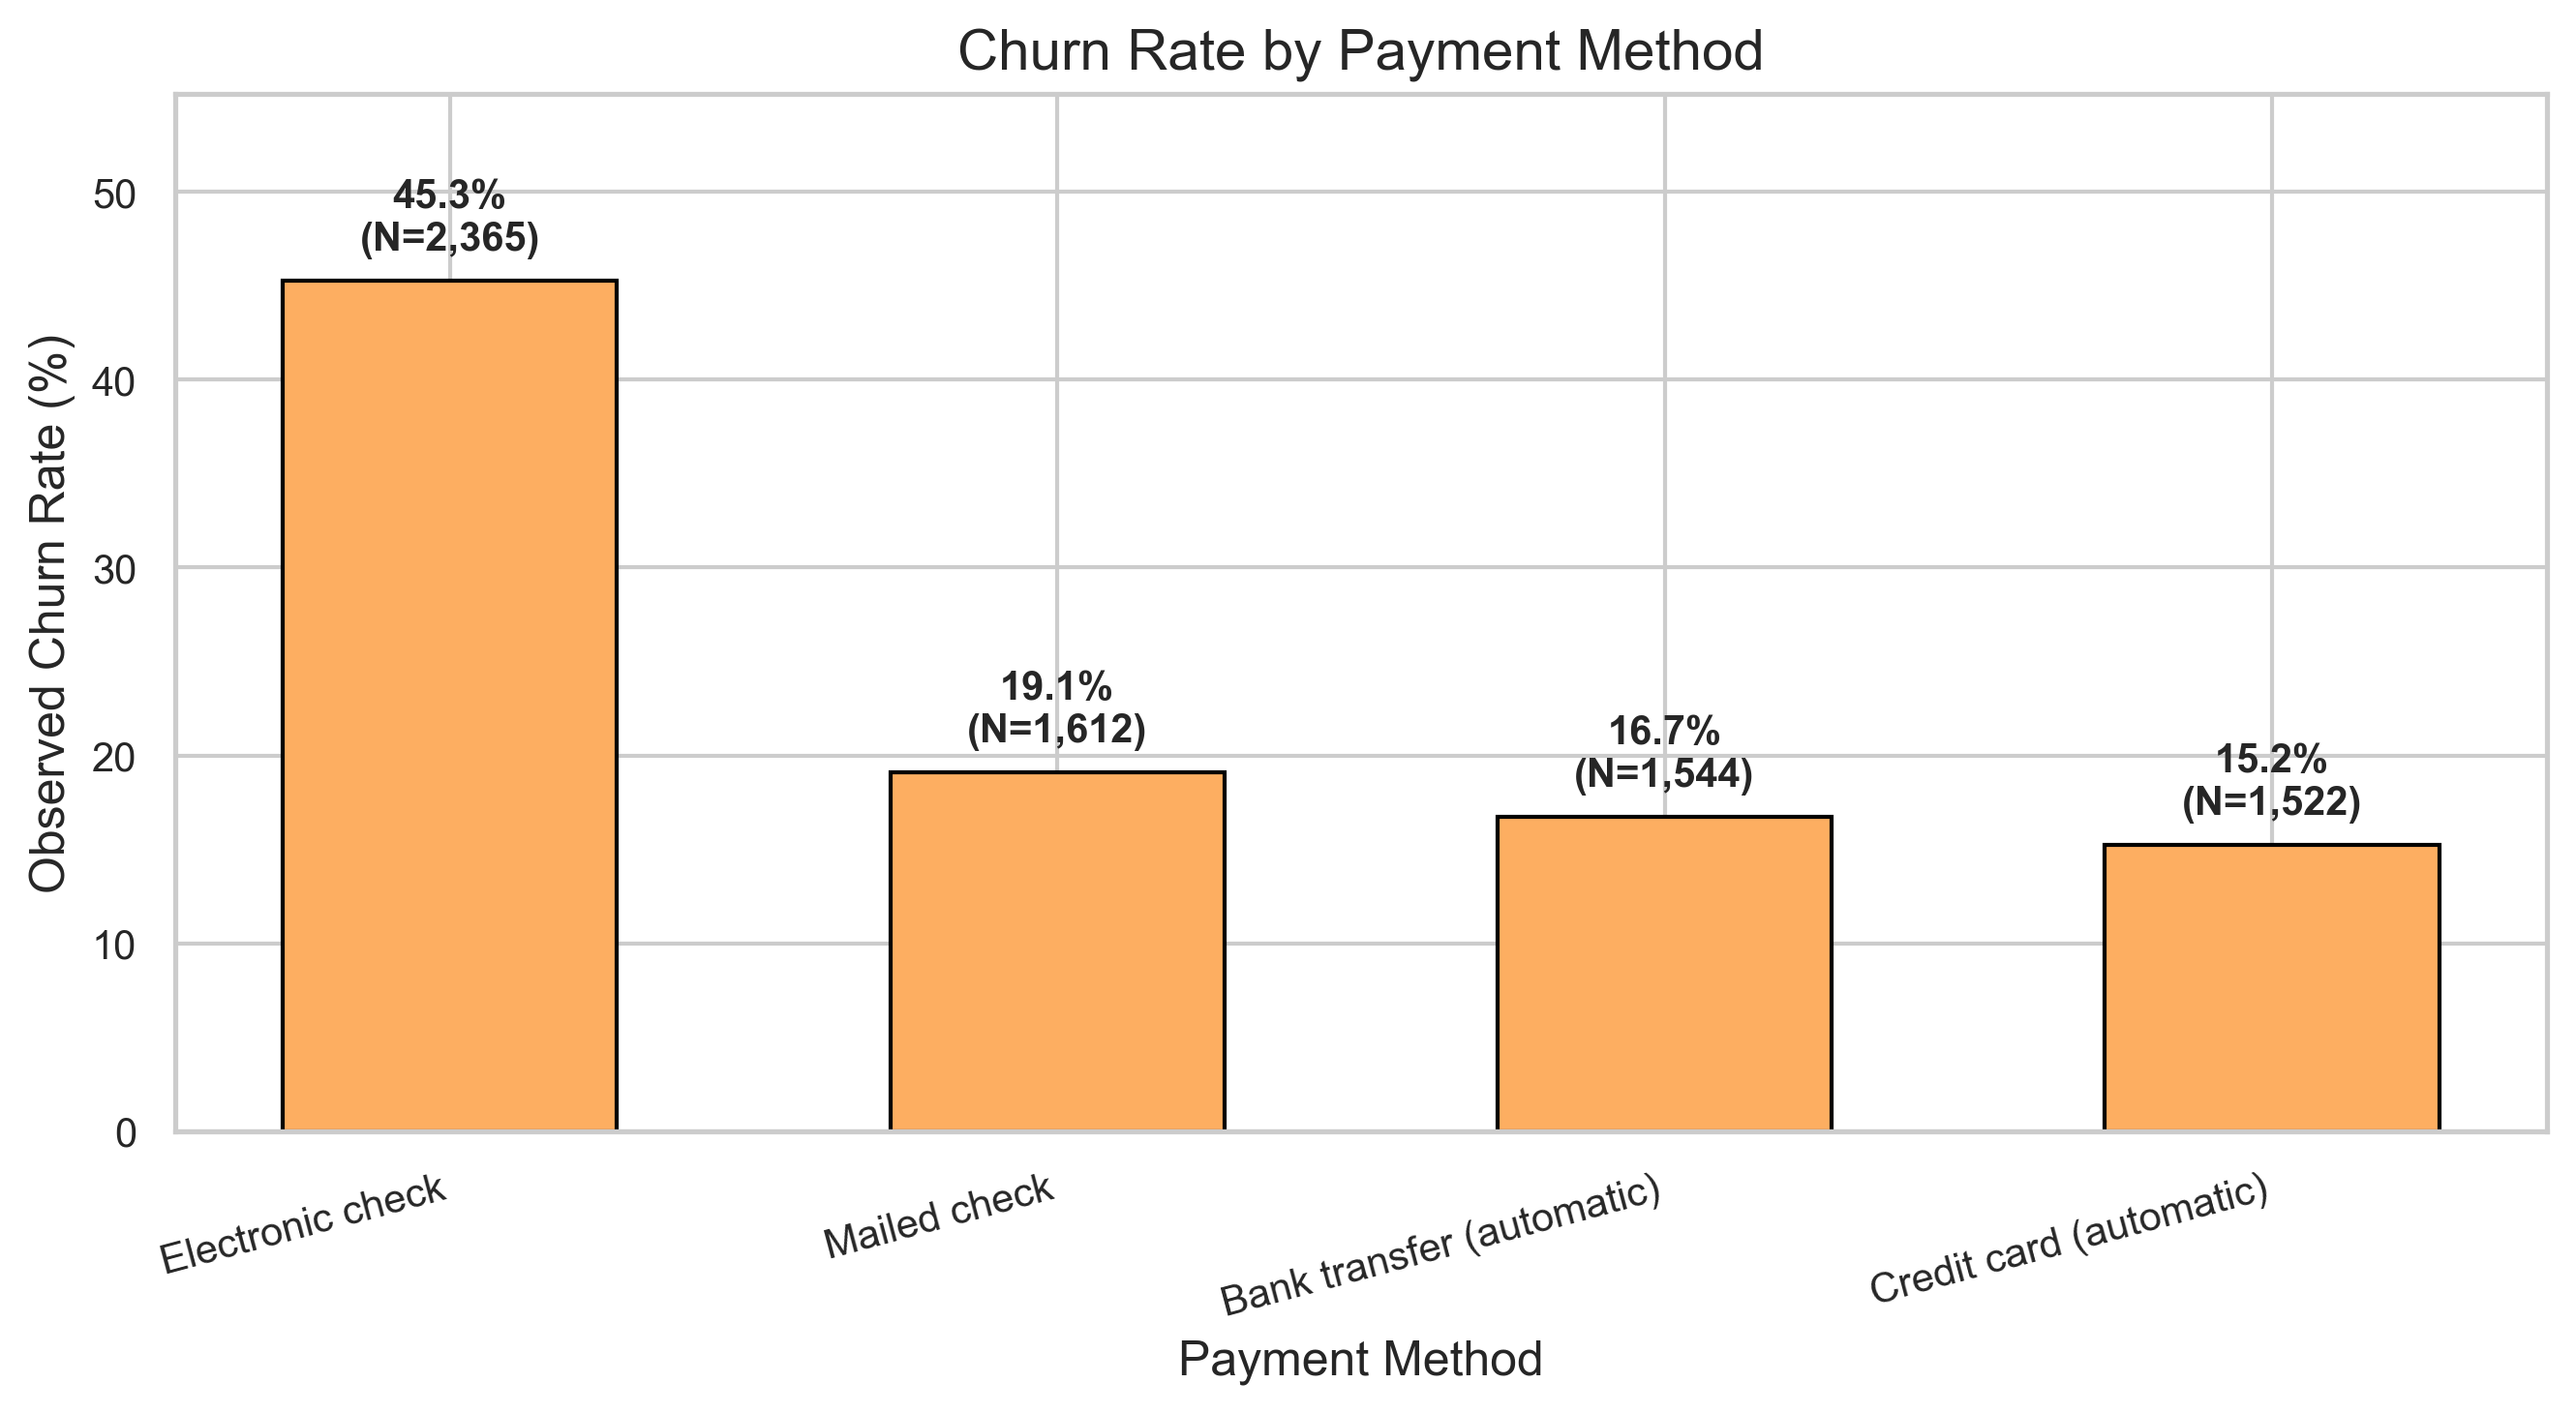
\includegraphics[width=\textwidth]{figures/eda_06_churn_by_payment_method.png}
        \caption{Churn Rate by Billing Payment Method}
        \label{fig:eda_payment}
    \end{subfigure}
    \caption{Exploratory Analysis of Billing Charges and Settlement Channels}
    \label{fig:eda_charges_payment}
\end{figure}

\section{MODEL BUILDING}
Model training is managed by \texttt{src/train\_models.py}. Each of the four primary classifiers is instantiated with fixed random seeds ($\texttt{random\_state}=42$) and evaluated through 5-fold stratified cross-validation on the training set prior to full training.
\begin{itemize}
    \item \textbf{Logistic Regression:} Trained in 2.44 seconds, achieving a mean cross-validated F1-score of $0.6285 \pm 0.0228$.
    \item \textbf{Support Vector Machine:} Trained in 235.25 seconds, achieving a mean cross-validated F1-score of $0.6236 \pm 0.0194$.
    \item \textbf{Random Forest:} Trained in 26.13 seconds, achieving a mean cross-validated F1-score of $0.6368 \pm 0.0160$.
    \item \textbf{Multi-Layer Perceptron:} Completed in 17 iterations (loss: 0.4008) in 64.39 seconds, achieving a mean cross-validated F1-score of $0.5735 \pm 0.0117$.
\end{itemize}
Trained model objects are saved to \texttt{models/*\_model.joblib}.

\section{EVALUATION PIPELINE AND CODE STRUCTURE}
Test evaluation is implemented in \texttt{src/evaluate\_models.py}. For each model, binary predictions and calibrated probability scores are generated for all 1,409 held-out test customers. Output files include:
\begin{itemize}
    \item \texttt{results/model\_comparison.csv}: Complete tabular metrics for all four classifiers.
    \item \texttt{results/predictions.csv}: Individual customer IDs, actual labels, and predicted probabilities.
    \item \texttt{results/confusion\_matrices/}: Detailed confusion matrix data for each model.
    \item \texttt{results/classification\_reports.json}: Class-level precision, recall, and support.
\end{itemize}

Listing~\ref{lst:pipeline_core} illustrates the core scikit-learn training, leakage prevention, and model evaluation pipeline implemented in the project.

\begin{lstlisting}[language=Python, caption={Core Implementation of the Leakage-Free ML Pipeline}, label={lst:pipeline_core}]
# Representative snippet from src/preprocessing.py and src/train_models.py
from sklearn.model_selection import train_test_split, StratifiedKFold, cross_val_score
from sklearn.compose import ColumnTransformer
from sklearn.pipeline import Pipeline
from sklearn.preprocessing import StandardScaler, OneHotEncoder
from sklearn.impute import SimpleImputer
from sklearn.ensemble import RandomForestClassifier

# 1. Stratified Train/Test Partition (80:20)
X_train_raw, X_test_raw, y_train, y_test = train_test_split(
    X, y, test_size=0.20, random_state=42, stratify=y
)

# 2. Build Preprocessor and Fit EXCLUSIVELY on Training Split
preprocessor = ColumnTransformer(
    transformers=[
        ("num", Pipeline([
            ("imputer", SimpleImputer(strategy="median")),
            ("scaler", StandardScaler())
        ]), NUMERIC_COLS),
        ("cat", Pipeline([
            ("imputer", SimpleImputer(strategy="most_frequent")),
            ("onehot", OneHotEncoder(handle_unknown="ignore", sparse_output=False))
        ]), CATEGORICAL_COLS)
    ]
)
X_train = preprocessor.fit_transform(X_train_raw)
X_test = preprocessor.transform(X_test_raw)  # Leak-free transformation

# 3. Train Classifier with Balanced Weighting
model = RandomForestClassifier(
    n_estimators=150, max_depth=10, min_samples_split=5,
    class_weight="balanced", random_state=42, n_jobs=1
)
model.fit(X_train, y_train)

# 4. Generate Predictions and Calibrated Probabilities on Held-Out Test Set
y_pred = model.predict(X_test)
y_prob = model.predict_proba(X_test)[:, 1]
\end{lstlisting}
